% Hoda Abbasi
% 16 March 2016

\documentclass[]{book}
\input Latex_macros/Definitionen.tex
\usepackage{a4}
\usepackage{graphicx}
\usepackage{tikz-qtree}
\usepackage[active]{srcltx}
\usepackage[all]{xy}
\usepackage{enumerate}

\setcounter{tocdepth}{4}
\setcounter{secnumdepth}{4}
\newcommand{\Schrift}{report}

\begin{document}
\title{Hardness measures of clause-sets}

\author{Hoda Abbasi\\
        PhD Candidate\\
        Computer Science Department\\
        Swansea University\\}
\maketitle

\tableofcontents
%%%%%%%%%%%%%%%%%%%%%%%%%%%%%%%%%%%%%%%%%%%%%%%%%%%%%%%%%%
\chapter{Introduction}
\label{cha:Introduction}

??????????????
%%%%%%%%%%%%%%%%%%%%%%%%%%%%%%%%%%%%%%%%%%%%%%%%%%%%%%%%%%
\chapter{Preliminaries}
\label{cha:Preliminaries}

\section{Clause-sets}
\label{sec:Clause-sets}

The infinite set of variables is denoted by $\Va$. A partial assignment $\vp$ is a map which assigns a unique value in $\set{0,1}$ to some elements of a finite set of variables. The domain of this map is a set of variables denoted by $\var(\vp)$. The set of all partial assignments is indicated by $\Pass$ and for $V \in \pote(\Va)$, $\Tass(V)$ is the set of total assignments over $V$. The empty partial assignment is denoted by $\epa:= \es \in \Pass$. For a partial assignment $\vp \in \Pass$, the number of variables is defined as $n(\vp):=\abs{\var(\vp)}$. For two partial assignments $\vp, \psi \in \Pass$, the composition operation is defined as $\vp \circ \psi := \psi \cup (\vp \sm \var(\psi)) \in \Pass$ which is the union of their variables if they do not conflict. In the case of conflicting variables, the second assignment is considered. This operation has associative property and it is commutative if $\vp, \psi$ do not clash.

A literal is a pair $(v,\ve)$ with $\var((v,\ve)):=v \in \Va$ (the underlying variable) and $\val((v,\ve)):=\ve \in \set{0,1}$. The set of all literals is $\Lit$. Two literals $x, y \in \Lit$ clash if they have a same variable but different values. For a set $L \sse \Lit$ we define $\var(L) := \set{\var(x) : x \in L}$, $\lit(L):= \set{x \in \Lit : \var(x) \in \var(L)}$ and $\ol{L} := \lit(L) \sm L$. A clause is defined as a finite and clash-free set of literals. The set of all clauses is denoted by $\Cl$ and $\bot := \es \in \Cl$ is the empty clause. The length (width) of a clause $C$ is the number of variables in $C$.

A clause-set is a finite set of clauses and $\Cls$ is the set of all clause-sets. The empty clause-set is indicated by $\top := \es \in \Cls$. For $F \in \Cls$ we define $\var(F) := \bc_{C \in F} \var(C) \in \pote(\Va)$ and $\lit(F) := \var(F) \cup \ol{\var(F)}$. The number of variables in $F$ is denoted by $n(F) := \abs{\var(F)} \in \NNZ$ and the number of clauses is $c(F) := \abs{F} \in \NNZ$. The number of literal occurrences in $F$ is also denoted by $\ell(F) := \sum_{C \in F} \abs{C} \in \NNZ$. If the union of literals occurring in $F$ is indicated by $\bigcup F \subset \Lit$, then a pure literal for $F \in \Cls$ is defined as $x \in \bigcup F$ and $\ol{x} \not \in \bigcup F$. A clause-set $F$ is called $k-\Cls$ if every clause in $F$ has length (width) at most $k$. A full clause $C$  for a clause-set $F$ is defined as $C \in F$ and $\var(C) = \var(F)$, and a clause-set $F$ is called full if every clause of $F$ is full. The full clause-set for a finite set of variables $V$ is denoted by $A(V)$. 

\begin{examp}\label{exp:An}
  If $A(V)$ for $V=\set{1,..., n}$ is indicated by $A_n$ then $A_0 = \set{\bot}$, $A_1 = \set{\set{1},\set{-1}}$ and $A_2 = \set{\set{-1,-2},\set{-1,2},\set{1,-2},\set{1,2}}$.
\end{examp}

Partial assignments are extended from variables to literals using $\vp(\ol{v})=\ol{\vp(v)}$. The operation of a partial assignment on a clause-set is defined as $\vp * F := \set{C \sm \vp : C \in F \wedge C \cap \ol{\vp} = \es} \in \Cls$. This means removing all clauses having at least one literal with $\vp (x)=1$ and then, removing from all clauses the literals with $\vp (x)=0$. For a clause $C$, the partial assignment $\vp_C$ sets precisely the literals in $C$ to 0. A clause-set $F$ is called satisfiable if there exists a partial assignment $\vp$ such that $\vp * F = \top$. Another definition for a satisfiable clause-set $F$ is that there exists a clause which clashes with all clauses of $F$. The set of all satisfiable clause-sets is indicated by $\Sat := \set{F \in \Cls \mb \ex\, \vp \in \Pass : \vp * F = \top}$ while $\Usat := \Cls \sm \Sat$. If $\vp * F = \top$ then the partial assignment is called a satisfying assignment for $F$.

A boolean function is a total assignment $f$ over a finite set of variables $V$ and denoted by $f:  \Tass(V) \ra \set{0,1}$. The Conjunctive Normal Form (or the CNF-representation) is the interpretation of a clause-set $F$ as a boolean function $f$ by considering the $F$ as the conjunction of clauses and a clause $C \in F$ as the disjunction of literals. In general, $F$ is a CNF-representation of $f$ if $\var(F) \spe \var(f)$ and for $\vp \in \Tass(\var(f))$, $(\vp * F) \in \Sat \Lra f(\vp) = 1$. If $v \in \var(f)$ it is called primary variable while $v \in \var(F) \sm \var(f)$ is called auxiliary variable.

\section{Implication-relation}
\label{sec:imprel}

The implication-relation for two clause-sets $F, F'$ is defined as $F \models F'$ if $\fa\, \vp \in \Pass : \vp * F = \top \Ra \vp * F' = \top$. This relation can also be considered between a clause $C$ and a clause-set $F$ if $F \models \set{C}$ (which is indicated as $F \models C$). For  $F \in \Usat$ the only implication-relation is $F \models \bot$. 

A literal $x$ is called forced literal for a clause-set $F$ if $F \models x$ and $\pab{x \ra 1}$ is the forced assignment for $F$. $\pab{x \ra 1} * F$ is satisfiability-equivalent to $F$. A clause $C$ is called an implicate of a clause-set $F$ if $F \models C$ and it is called a prime implicate if there no $ C' \sse C$ as an implicate of $F$. The set of all prime implicates of $F$ is denoted by $\primec_0(F) \in \Cls$. A clause $C$ is called an implicant of a clause-set $F$ if $C$ as a partial assignment is a satisfying assignment for $F$. In other words, $C$ must fulfill $C * F=\top$. A prime implicant is a minimal implicant and the set of all prime implicants is indicated by $\primec_1(F) \in \Cls$. For example, for $F \in \Usat$ we have $\primec_0(F) = \set{\bot}$ and $\primec_1(F) = \top$.

\begin{examp}\label{exp:bbb}
For $F = \{\{ \ol x, y\} , \{ \ol y, z\}\}, prc_0(F) = \{\{\ol x, y\} , \{\ol y, z\} , \{\ol x, z\}\}$. Also for $F = \set{\set{x, y} , \set{x,\ol y}}, prc_0(F) = \set{\set{x}}$.
\end{examp}

Two clause-sets $F, G$ are called logically equivalent if $F \models G$ and $G \models F$. In this case, we have $\primec_0(F) = \primec_0(G)$ and $\primec_1(F) = \primec_1(G)$.

\section{Resolution}
\label{sec:Resolution}

The resolution is an operation applied to two clauses $C,D$ which clash in exactly one variable and produces a new clause. The result of the resolution for $C \cap \overline D = \{ x \}$ (which is called resolvent) is defined as $C \diamond D := (C \cup D) \setminus \{x, \overline x\} $. $C,D$ are called resolvable clauses and $x$ is the resolution literal.

A full binary tree is a tree that each node (except leaves) has exactly two children (or parents). Using the resolution operation, a binary tree is produced for a clause-set $F$ which is called the resolution tree. The tree is indicated by $T : F \vdash C$ which clause $C$ is the root (conclusion) of $T$. The leaves of $T$ (axioms) are the clauses of $F$ and each inner node is the resolvent of its two parents. The number of nodes in $T$ is called tree-resolution complexity and denoted by $\comptr(R) \in \NN$. A resolution proof of a clause $C$ from a clause-set $F$ is a resolution tree $T : F \vdash C$. If a resolution proof drives $\bot$, it is called a resolution refutation and $F$ is unsatisfiable.

If a clause $C$ is an implicate of a clause-set $F$, then there is a resolution tree $T : F \vdash C$. A clause $C$ is a prime implicate for $F$ iff there is no tree $T': F \vdash C'$ for some $C \sst C'$.

\begin{examp}\label{exp:res1}
A resolution tree for $F = \set{\set{a,b},\set{\ol a,b},\set{a, \ol b},\set{\ol a, \ol b}}$ is as Fig \ref{fig:resol1}. Since the empty clause is driven, it is called resolution refutation.
	   \begin{figure}
	   \centering  
       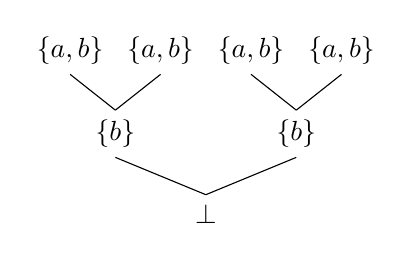
\begin{tikzpicture}[grow'=up]
       \Tree [.$\bot$  [.${\{b\}}$ ${\{a,b\}}$ ${\{\ol a,b\}}$ ] [.${\{ \ol b\}}$ ${\{a, \ol b\}}$ ${\{\ol a, \ol b\}}$ ] ]
       \end{tikzpicture}
	   \caption{A resolution tree for Example \ref{exp:res1}.}
	   \label{fig:resol1}
       \end{figure}
\end{examp}

For a resolution proof $T: F \vdash C$ consider that each node (resolvent) in $T$ have at least one parent with length at most $k$. In this case, the resolvent is called $k$-resolvent. If every resolvent in $T$ is a $k$-resolvent, then $T:F \vdash C$ is called $k$-resolution and denoted by $F \vdash^k C$. For example, 1-resolution is the unit resolution.
%If a $k$-resolution refutation exists then the unsatisfiability can be proved by the unit-preference strategy within k levels and vice versa \cite{h19}.

\section{Generalised unit-clause propagation}
\label{sec:rkred}

A reduction is considered as a map $r: \Cls \ra \Cls$ such that for all $F \in \Cls$, $r(F)$ is satisfiability-equivalent to $F$. Using the reduction technique, unsatisfiability is resulted if $\bot \in r(F)$. An example of the reduction is unit resolution (or unit propagation) which is applied to a clause-set $F$ with at least one unit-clause (a clause with one literal). This technique is performed by setting the literal in unit-clause to its satisfying assignment. For example for clause $\set{x}$, we set the literal $x$ to true. If the reduction yields $\bot$, then $F$ is unsatisfiable. Else, if there are more unit-clauses, this step is continued until no unit-clause is left.

Another case of the reduction is generalised unit-clause propagation introduced in \cite{h10} and denoted by $\rk_k$. This technique removes some forced literals using forced assignments and discovers unsatisfiability if $\bot \in \rk_k(F)$. If $\bot \not \in F$, it starts from $k=1$ and increases $k$ in each step. For $k=1$, the generalised unit-clause propagation eliminates all unit-clauses with assigning their satisfying assignment. Thus, $\rk_1$ is the unit-clause propagation and two cases may happen:  $\rk_1 \in \set{\set{\bot},\top}$ or all clauses in $\rk_1$ must have length at least $2$. In the second case, the next step is to obtain $\rk_2$ which is called failed literal elimination since all unit-clauses have already been removed. In each step $k$, if $\rk_k$ yields $\bot$ then the original clause-set $F$ is unsatisfiable while $F$ is satisfiable if $\top$ is obtained. In the latter case, the sequence of forced assignments eliminated until that level is a satisfying assignment for $F$.

The map $\rk_k$ is well-defined since it does not depend on the choices of literals in each step. For example, in the process of obtaining  $\rk_1$ the final result does not change based on the order of choosing the unit literals. For all clauses $C \in F$ if $\abs{C} > k$, then $\rk_k(F) = F$. This means that this technique is not complete since $\rk_k(F)$ can not discover the unsatisfiability of a clause-set $F$ if all clauses in $F$ have length at least $K+1$.

\begin{defi}\label{def:rk}
\cite{h10} The maps $\rk_k: \Cls \ra \Cls$ for $k \in \NNZ$ are defined as follows (for $F \in \Cls$):
  \begin{eqnarray*}
  \rk_0(F) & := &
  \begin{cases}
  \set{\bot} & \text{if } \bot \in F\\ F & \text{otherwise}
  \end{cases}\\
  \rk_{k+1}(F) & := &
  \begin{cases}
  \rk_{k+1}(\pao x1 * F) & \text{if } \ex\, x \in \lit(F) : \rk_k(\pao x0 * F) = \set{\bot}\\ F & \text{otherwise}
  \end{cases}.
  \end{eqnarray*}
\end{defi}

\begin{examp}\label{exp:rk}
Using literals $a,b,c,d$, $\rk_k(F)$ for some examples is computed as follows:
  \begin{enumerate}
  \item $\rk_k(\set{\bot}) = \set{\bot}$ for $k \ge 0$ and $\rk_k(\top) = \top$ for $k \ge 0$.
  \item For $F := \set{\set{a},\set{b},\set{c},\set{d}}$: $\rk_0(F) = F$, $\rk_k(F) = \top$ for $k \ge 1$.
  \item For $F := \set{\set{a,b},\set{a,\ol{b}}, \set{\ol{a},b},\set{\ol{a},\ol{b}}}$: $\rk_k(F) = F$ for $k \le 1$, $\rk_k(F) = \set{\bot}$ for $k \ge 2$.
  \end{enumerate}
\end{examp}

\section{Horton-Strahler number}
\label{sec:hs}

The Horton-Strahler number is a measure of branching complexity for trees. Here, the Horton-Strahler number is defined for a resolution tree $T$ and denoted by $\hts(T) \in \NNZ$. To obtain $\hts(T)$, we start with leaves (axioms) whose Horton-Strahler number are defined as $\hts(T) := 0$. Then, for each inner node with two children $T_1, T_2$, we have two cases. If $\hts(T_1)= \hts(T_2)$, then $\hts(T) := \hts(T_1)+ 1$. Otherwise, $\hts(T) := \max(\hts(T_1),\hts(T_2))$. This means that the Horton-Strahler number for each node is the shortest distance from that node to the leaves. For example, for all resolution trees $T:F \vdash \bot$ with $\hts(T) \leq 1$, every node is a leaf or has a leaf as a child.

%%%%%%%%%%%%%%%%%%%%%%%%%%%%%%%%%%%%%%%%%%%%%%%%%%%%%%%%%%
\chapter{Hardness measures}
\label{cha:Hardness Measures}

The hardness is defined as a measure of complexity (the amount of effort needed to discover unsatisfiability) for a representation $F$ of a boolean function $f$ in SAT solving. Various hardness measures have been investigated in the literature and the relation between these measures is studied in \cite{h5},\cite{h18},\cite{h8}. In this report, two measures of the hardness are investigated. The first one is the tree-hardness which is related to the size of resolution proofs. The width-hardness is the second measure and is related to the width of clauses in resolution proofs. We start with defining these measures for unsatisfiable clause-sets and then, we extend the definitions to the satisfiable clause-sets. 

\section{Tree-hardness of clause-sets}
\label{sec:Hardnessunsat}

For an unsatisfiable clause-set $F$ there exist a resolution refutation $T:F \vdash \bot$ with the Horton-Strahler number $\hts(T)$. The tree-hardness (or just hardness) for $F \in \Usat$ is defined as the minimum of $\hts(T)$ of all  $T:F \vdash \bot$ and denoted by $\hardness(F)$. This means that the hardness of $F$ is the $\hts(T)$ of the biggest full binary tree which can be embedded into each $T : F \vdash \bot$. From computational point of view, it is not a practical method to obtain the hardness. Thus, another definition is defined using the generalised unit-clause propagation $\rk_k$ which is the minimum of $k \in \NNZ$ such that $\rk_k(F)$ yields $\bot$. It should be noted that $\rk_k$ can not yield $\set{\bot}$ if all clauses in $F$ have length at least $K+1$.

\begin{examp}\label{exp:harducls}
For $\set{\set{x,y},\set{x,\ol{y}},\set{\ol{x},y},\set{\ol{x},\ol{y}}}$ we have $r_1(F)=F, r_2(F)=r_2( \langle a \rightarrow 1 \rangle * F) = \{ \bot \}$(since $r_1( \langle a \rightarrow 0 \rangle * F)=r_1 (\{\{ b \}, \{ \ol b \}\}) = \{ \bot \}$). Thus, $\hardness(F) = 2$. In general, the hardness of full clause-sets are as $\hardness(A_n)=n$.
  
Following, $\hardness(F)$ for some more examples of unsatisfiable clause-sets $(F)$ are computed:
  \begin{enumerate}
  \item $\hardness(F) = 0$ if $\bot \in F$.
  \item $\hardness(\set{\set{a},\set{\ol{a}}}) = 1$.
  \item $\hardness(\set{\set{a},\set{\ol{a},b}, \set{\ol{b},c}, \set{\ol{c}}}) = 1$. 
  %In general, Horn clause-sets (whose clauses have at most one positive literal) have hardness one.
  \item $\hardness(\set{\set{a,\ol{b}},\set{\ol{a},b},\set{b,\ol{c}},\set{\ol{b},c},\set{a,b,c},\set{\ol{a},\ol{b},\ol{c}}}) = 2$.
  \end{enumerate}
\end{examp}

Each satisfiable clause-set $F \in \Cls \sm \set{\top}$ can be converted to an unsatisfiable clause-set by applying a partial assignment $\vp$. For extending the hardness measure to a satisfiable clause-set, we should consider the worst case value of $\hardness$ for $\vp * F \in \Usat$ which is the maximum of $\hardness(\vp * F)$. The reason is that $\hardness(\vp * F) \leq \hardness(F)$ (the application of a partial assignment on $F$ do not increase the hardness) and one can easily find a $\vp$ such that $\bot \in \vp * F$ and $\hardness(\vp * F)=0$. For $\vp$ we only need to consider the minimal partial assignment which is $\vp_C : C \in \primec_0(F)$. For $F = \top$, since it is not convertible to an unsatisfiable clause-set, we assign the minimum of the hardness which is zero.

\begin{defi}\label{def:hd-extended}
The hardness is a map that assigns a natural number for a representation of a boolean function $f$ as a clause-set $F \in \Cls$ and is denoted by $\hardness : \Cls \rightarrow \NNZ$. To obtain the hardness of  $F$, there are three cases: if $F = \top$, then $\hardness(F) := 0$. Else if $F \in \Usat$, then $\hardness(F) := \min \set{k \in \NNZ : \rk_k(F)=\set{\bot}}$. Otherwise, $F \in \Sat \sm \set{\top}$ and $\hardness(F) := \max \set{ \hardness(\vp * F) : \vp * F \in \Usat }$.
\end{defi}

\begin{examp}\label{exp:hd-extd}
For $F = \set{\set{x, y} , \set{x,\ol y}} \in \Sat$ with $\primec_0(F) = \set{\set{x}}$,  $\hardness(F)= \max \set{ \hardness(\vp * F) : \vp =\pab{x \ra 0} }=\hardness(\set{\set{y},\set{\ol y}})=1$.
\end{examp}

\begin{lem}\label{lem:hd-dec}

\end{lem}
\begin{prf}
The existence of $v$ and $\ve$
\end{prf}

\section{Width-hardness of clause-sets}
\label{sec:whdd}

Another measure for complexity of an unsatisfiable clause-set $F$ is the width-hardness (or asymmetric width) and indicated by $\whardness(F)$. For each $F \in \Usat$ there exist a resolution refutation $T:F \vdash \bot$. If each node of $T$ is a $k$-resolvent, then the tree is a $k$-resolution tree. The width-hardness of $F$ is the minimum of $k$ for all $k$-resolution trees $T:F \vdash \bot$. This definition is extended for a satisfiable clause-set $F$ by considering the worst case (maximum) of the width-hardness for the extended $F$ (that is $ \vp * F \in \Usat$) and $\whardness(\top):=0$.

\begin{defi}\label{def:whd-extended}
The width-hardness is a map denoted by $\whardness : \Cls \rightarrow \NNZ$ for a representation of a boolean function $f$ as a clause-set $F \in \Cls$. To obtain the width-hardness of  $F$, there are three cases: if $F = \top$, then $\whardness(F) := 0$. Else if $F \in \Usat$, then $\whardness(F) := \min \set{k \in \NNZ : F \vdash^k \bot}$. Otherwise, $F \in \Sat \sm \set{\top}$, and $\whardness(F) := \max \set{ \whardness(\vp * F) : \vp * F \in \Usat }$.
\end{defi}

For example if $\bot \in F$, then $F \vdash^0 \bot$ and $\whardness(F)=0$. Also if $\rk_1(F)=\set{\bot}$, then it is 1-resolution (unit resolution) and  $\whardness(F)=1$.

\section{Game characterisations of hardness measures}
\label{sec:game-pd}

In \cite{h18}, a game is characterised to obtain $\hardness(F)$ or $\whardness(F)$ of a clause-set $F \in \Cls$ called Prover-Delayer game (or the hardness game). The game is performed between two payers, Prover and Delayer. Delayer starts the game and two players play in turns. There is a partial assignment $\vp: \var(\vp) \in F$ (initially empty) that is extended in each turn by the two players. Therefore, in each turn a new clause-set $F'$ is obtained by assigning at most one variable in $\vp$ with $\hardness(F')$ (or $\whardness(F')$). The game ends when ????????

First, we consider the game for $\hardness(F)$. In this case, Delayer claims to know a partial assignment $\vp$ such that ?????
The game is continued until all variables in $F$ are assigned and one of $\vp * F = \top$ or $ \bot \in \vp * F$ is achieved. ????????

Prover must decrease exactly one unit of $\hardness(F)$. ????????????



\begin{lem}\label{lem:game1}
The game is well-defined since it does not depend on choices.
\end{lem}

\begin{defi}\label{def:atomic-move}
The atomic move in the delayer-prover game is the extension of the partial assignment $\vp$ for the clause-set $F$. In the case of Delayer, the atomic move is???

In the case of Prover, the atomic move is assigning exactly one variable $v \in \var(F)$ (which is extending $\vp$ with exactly one assignment) and decreasing hd??????????????
\end{defi}

Delayer wants to maximize the hardness. Since the operation of a partial assignment does not increase the hardness, the optimal move for Delayer is ???????????
%%%%%%%%%%%%%%%%%%%%%%%%%%%%%%%%%%%%%%%%%%%%%%%%%%%%%%%%%%
\chapter{The hardness measures for Tseitin graph}
\label{cha:hdgame}

\section{XOR representation}
\label{sec:XOR representation}
For representing a boolean function $f$ we defined CNF-clause-sets in Section \ref{sec:Clause-sets}. Here, another representation of $f$ is introduced (called XOR-representation) which is used for extending the hardness game for graphs. An XOR-clause-set for $f$ is the interpretation of a clause-set $F \in \Cls$ as a system of XOR-constraints whose clauses $C$ are parity equation for $v \in \var(C)$. 


\begin{defi}\label{def:xor-const} 
An XOR-constraint (or parity constraint) is a boolean function (parity function) $f$ in the form of $x_1 \oplus \dots \oplus x_n = \ve$ that $x_1, \dots, x_n \in \Lit$ and $\ve \in \set{0,1}$. Two XOR-constraints $f_1, f_2$ are equivalent iff $\var(f_1) = \var(f_2)$ and both have the same parity for literals.
\end{defi}
Remarks:
\begin{enumerate}
      \item $x_1 \oplus \dots \oplus x_n = y$ is equivalent to $x_1 \oplus \dots \oplus x_n \oplus y = 0$
      \item $x \oplus x = 0$, $x \oplus \ol{x} = 1$, $0 \oplus x = x$, $1 \oplus x = \ol{x}$.
\end{enumerate}

\begin{defi}\label{def:xor-cls}
An XOR-clause $C \in \Cl$ with literal $x \in \Lit$ is an XOR-constraint with $\oplus_{x \in C} = 0$. Thus, two XOR-clauses $C, D$ are equivalent iff $\var(C) = \var(D)$ and both with the same parity. In an XOR-clause, there is no repetitive literals since $x \oplus x = 0$. In the case of clashing literals, we remove them using the laws $x \oplus \ol{x} = 1$ and $1 \oplus y = \ol{y}$ (since according to the definition, clashing literals are not allowed in clauses).

An XOR-clause-set is a clause-set $F \in \Cls$ whose clauses $C$ are interpreted as an XOR-clause.  


\end{defi} 

The operation of a partial assignment $\vp \in \Pass$ to XOR-clause-sets is defined as the same definition for CNF-clause-sets. An XOR-clause-set $F$ is satisfiable if there exist a partial assignment $\vp$ such that $\var(\vp) \supseteq \var(F)$ and for every $C \in F$ the number of $x \in C$ with $\vp(x) = 1$ is even (that satisfies the equation  $\oplus_{x \in C} = 0$). 

The satisfiability of a CNF-clause-set is investigated using the resolution operation. Here, for investigating whether an XOR-clause-set is satisfiable or not, an operation is defined which is called XOR-sum over clauses of $F$ and denoted by $\oplus F \in \Cl$. This operation is applied to two XOR-clauses and produces a new clause or the result is inconsistent. The operation is performed as follows. If there are four literals as $x,\ol{x},y,\ol{y}$ for $x \ne y$, the XOR-sum of them is as $x \oplus \ol{x} = 1$ and $y \oplus \ol{y} = 1$. Thus, $1 \oplus 1 = 0$ and they are removed. If no clash remains, then the result is obtained as a clause $E \in \Cl$. Else if there is just one clash for literals $x, \ol{x}$ with at least one other literal $y$, then $x \oplus \ol{x} = 1$ and $1 \oplus y=\ol{y}$ and a new clause $E \in \Cl$ is obtained. Otherwise, if two literals $x, \ol{x}$ remains, then $\oplus F$ is called inconsistent. An XOR-clause-set $F \in \Cls$ is unsatisfiable if and only if there is $F' \sse F$ such that $\oplus F'$ is inconsistent.

\begin{examp}\label{exp:xorcls}
The satisfiability of the following XOR-clause-sets $F$ are investigated using the XOR-sum over clauses of $F$.
  \begin{enumerate}
  \item For $F=\top$, $ \oplus(F)= \oplus(\set{\bot})=\bot$ and $F$ is satisfiable.
  \item For $F=\set{\set{a,b},\set{b,c,\ol d}}$, $ \oplus(F) = \set{a,c,\ol d}$ and $F$ is satisfiable.
  \item For $F=\set{\set{a,b,c},\set{a, \ol b, \ol c}}$, $ \oplus(F) = \bot$ and $F$ is satisfiable.  
  \item  For $F=\set{\set{a,b},\set{a, \ol b},\set{c,d}}$, $\oplus (F)$ is inconsistent and $F$is unsatisfiable.
  \end{enumerate}
\end{examp}

For each XOR-clause-set $F$ there is a unique equivalent CNF-clause-set $F'$ (without auxiliary variables). To obtain this equivalent CNF-clause-set, a translation is defined and indicated by $X_0(F)$. This translation, converts each clause of $F$ to a set of full clauses in CNF-representation and then $F'$ is the union of these sets. If $F$ has long clauses, then obtaining $X_0(F)$ is not practical.

\begin{defi}\label{def:x0tr}
The $X_0$ translation is a map $X_0: \Cls \ra \Cls$ where the input is an XOR-clause-set and the output is a  CNF-clause-set. Consider an XOR-clause $C \in F$, the $X_0$ translation of this clause is defined as the set of prime implicates of the boolean function for $C$ (without auxiliary variables) and indicated by $X_0(C)=\primec_0(x_1 \oplus \dots \oplus x_n = 0)$. The translation $X_0(C)$ contains all the full clauses over the set of variables in $C$ whose parity are different from the parity of $C$. Thus, $\abs{X_0(C)}=2^{\var(C)-1}$. Finally, the CNF-clause-set is obtained by $X_0(F) := \bc_{C \in F} X_0(C)$.
\end{defi} 

\begin{examp}\label{exp:X0}
   For $F=\set{\set{a,\ol b}}$, $X_0(F)= \set{\set{a,b},\set{\ol a,\ol b}}$ and for $F=\set{\set{a},\set{b,c}}$, $X_0(F)=\set{\set{\ol a},\set{\ol a, b}, \set{a, \ol b}}$.
\end{examp}

\section{Tseitin graph}
\label{sec:Tseitin graph}

For extending the hardness game for graphs, first we need to describe Tseitin graph and Tseitin clause-set. A simple graph is a pair $G = (V,E)$ where $V$ is the set of vertices and $E$ is the set of edges. If we consider the graph as a triple $G = (V,E,\eta)$ such that $V$ is the set of vertices, $E$ is the set of edge-labels and $\eta: E \ra \set{e \sse V : 1 \le \abs{e} \le 2}$, we can describe parallel edges and loops. 

Consider a connected graph $G=(V,E,\eta)$ without loop. First, we label each edge with a distinct literal $x \in E$. Then, if we assign a charge $\rho$ to each vertex such that $\rho: V \ra \set{0,1}$, we obtain a unique XOR-clause-set corresponded to $G$. In this case, each vertex $w \in V$ is specified as an XOR-clause $C \in \Cl$ such that $\oplus_{x \in E, w \in \eta(x)} \; x = \rho(w)$. Then, the XOR-clause-set for $G$ is obtained by $T_0(G,\rho) := \set{C_w : w \in V} \in \Cls$. 

\begin{lem}\label{lem:chgvar}
Suppose that $T_0(G,\rho)$ is an XOR-clause-set for a graph $G=(V,E,\eta)$ without loop. We define $\Phi$ as an XOR-constraint for charges of vertices that is $\oplus_{w \in V} \rho(w) = \ve$ and $\ve \in \set{0,1}$. By assigning a value to all edges $x \in E$, we obtain $\rho(w)$ of all vertices and then, the value of $\ve$ in $\Phi$. In this case, if we change the value of an edge $x$, then $\rho(w)$ for each endpoint of $x$ must be changed to remain $\Phi$ unchanged.
\end{lem}
\begin{prf}
According to the definition, each vertex $w$ of $G$ is an XOR-clause with $\rho(w)$ such that  $\oplus_{x \in E, w \in \eta(x)} \; x = \rho(w)$ ($\rho$ is the parity). Since each literal corresponds to an edge connected to two vertices $w_1, w_2$, changing the value of a literal $x$ will change the parity $\rho(w)$ for equation of $w_1, w_2$. XXX
\end{prf}

For a graph such as Lemma \ref{lem:chgvar} with $\Phi$, if $\ve=0$ then we need to investigate the satisfiability of each XOR-clause to determine whether $T_0(G,\rho)$ is satisfiable or not. Else if $\ve=1$, $T_0(G,\rho)$ is unsatisfiable. The reason is as follows. If $\ve=1$ in $\Phi$, there is at least one vertex $w$ (XOR-clause $C$) with $ \rho(w) =1$ and according to the definitions in Section \ref{sec:XOR representation}, an XOR-clause $C$ is satisfiable if $\oplus_{x \in C} = 0$. Thus, $\oplus_{x \in C} = \rho(w) \not =0$ and $T_0(G,\rho)$ is unsatisfiable.

A graph $G$ as explained in Lemma \ref{lem:chgvar} with $\ve=1$ in $\Phi$, is called Tseitin graph. The equivalent CNF-clause-set of $G$ is obtained by $X_0$ translation of $T_0(G,\rho)$ and indicated by $T(G,\rho) := X_0(T_0(G,\rho))$. The clause-set $T(G,\rho) \in \Usat$ is called Tseitin clause-set of $G$.

\section{Game-tree}
\label{sec:Game-tree}

For each Tseitin clause-set $F$ corresponding to a Tseitin graph $G$, there exist a unique tree called game-tree such that shows all possible atomic moves for Prover and Delayer. The tree is upside down with even number of levels and the root of the tree is $F$. Each node of the game-tree (except leaves) corresponds to a clause-set $F'$ ($ \bot \not \in F'$) whose variable is at most one unit less that the upper-level nodes. The children of each node are the all possible atomic moves in that round. Each path from root must end in a leaf since the edges of graph (which correspond to the maximum of atomic moves of Prover) are finite and the leaves correspond to $\bot$. ????????The hardness of $F$ is achieved by assigning a number to each node (starting from leaves) and obtaining the number of the root.

To obtain the harness, first we assign a number to each leaf that corresponds to the scores of Prover (the number of Prover's atomic moves) through the path to that leaf. Since the last round of game is always played by Prover, we assign the minimum number of leaves to their parents (upper-level nodes). Then, we consider the upper level which is played by Delayer and therefore, we assign the maximum number of nodes for their parents. This process is continued until we get the root and and we assign the maximum number of root's children to the root (since the first round is played by delayer). Finally, the hardness of $F$ corresponds to the number of the root.

\begin{lem}\label{lem:game2}
For each arbitrary clause-set $F \in \Usat$, the game-tree is unique.
\end{lem}
\begin{prf}
??????????
\end{prf}
\begin{examp}\label{exp:gg1}
Fig \ref{fig:gg1} shows the game-tree for graph $K_3$. The children of each node are all possible moves (whether the move is optimal or not) in hardness game for $K_3$. Here, $\ve $ shows the empty move (or when delayer decides to do nothing) and $\bot$ shows the end of game. We start from leaves by counting the number of prover's moves until that leaf and assign this number to that leaf. 
\begin{figure}
\begin{center}
\includegraphics[scale =0.45]{gg1.png}
 \caption{The game-tree for $K_3$.}
\label{fig:gg1}
\end{center}
\end{figure}
\end{examp}

\section{Game characterisations for Tseitin graph}
\label{sec:hd-game-graph}

Consider an unsatisfiable Tseitin clause-set $T(G,\rho)$.

%lemma yyy  if we remove an edge, then \rho(w) of endpoints will change?????? proof: we know that f is unsatisfiable thus $\ve=1$ for $\Phi$. thus based on lemma xxx, too keep $\ve=1$ unchanged, if we remove any edge by assigning a value, then the equation of endpoints must be changed

%%%%%%%%%%%%%%%%%%%%%%%%%%%%%%%%%%%%%%%%%%%%%%%%%%%%%%%%%%
%\chapter{Conclusion and open problems}
%\label{cha:concl}

%%%%%%%%%%%%%%%%%%%%%%%%%%%%%%%%%%%%%%%%%%%%%%%%%%%%%%%%%%
\newpage
\bibliographystyle{plainurl}
\bibliography{HA_ResearchRef}

\end{document}

